\subsection{Induzione di Faraday}
Per l'acquisizione delle forme d'onda vengono prese le medesime accortezze della sezione precedente.
\begin{figure}[h]
    \centering
    \begin{minipage}{0.5\textwidth}
        \centering
        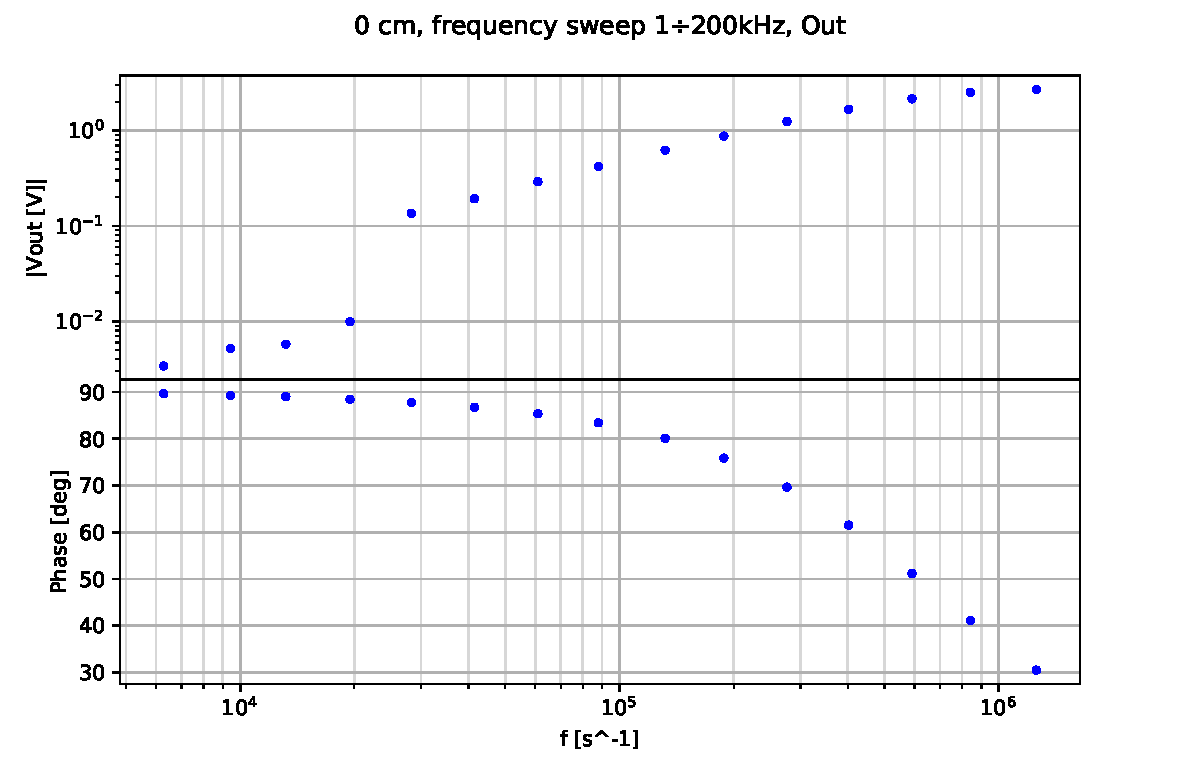
\includegraphics[width=\textwidth]{Figure_13.pdf} 
        %\caption{first figure}
    \end{minipage}\hfill
    \begin{minipage}{0.5\textwidth}
        \centering
        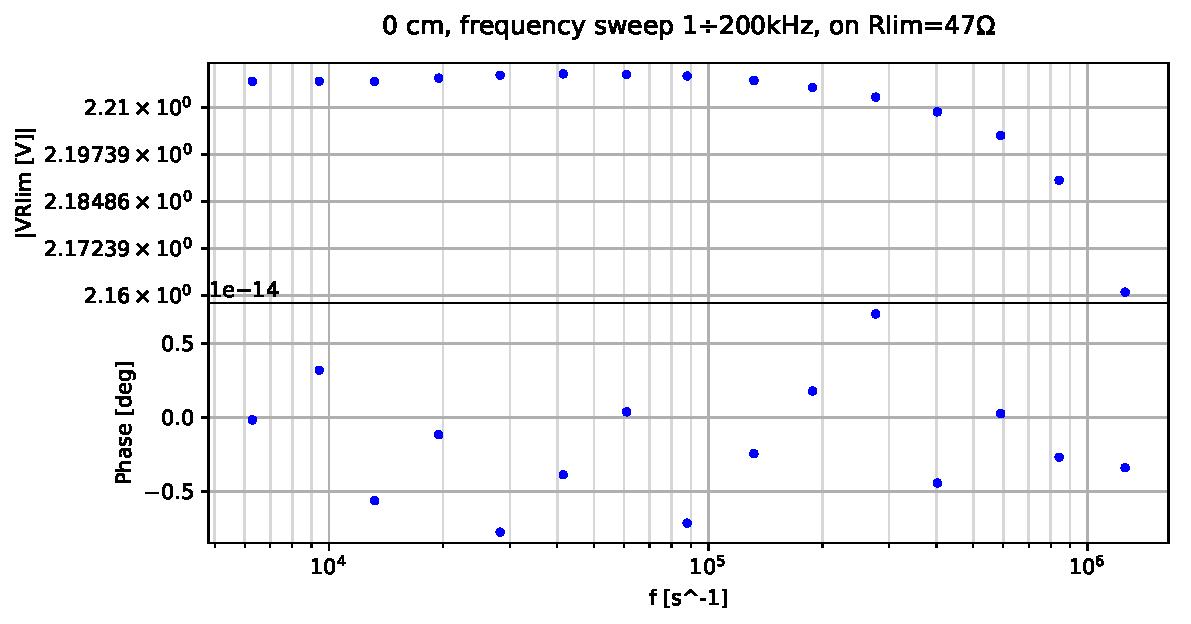
\includegraphics[width=\textwidth]{Figure_14.pdf} 
        %\caption{second figure}
    \end{minipage}
    \caption{Ampiezza dell'induzione e della corrente sulla sorgente al variare della frequenza.}
    \label{fig:induz}
\end{figure}
Dati i plot dei dati raccolti in figura \ref{fig:induz} si pu\'o procedere a calcolare il coefficiente di mutua induzione tra bobina sorgente e ricevente definendo $\epsilon_R$ la f.e.m. ai capi della ricevente in ingresso all'amplificatore e $i_S$ la corrente che scorre nella bobina sorgente misurata sapendo la tensione ai capi di $R_{lim}$:
\begin{gather}
	Z_{eff}(\omega) = \frac{\epsilon_R(\omega)}{i_S(\omega)}= \frac{V_{out}(\omega)}{G_{diff}(\omega) i_S(\omega)} \\
\end{gather}
Supponendo poi che l'accoppiamento sia di tipo induttivo, si pu\'o porre:
\begin{gather}
	Z_{eff}(\omega)=j \omega M_{RS} \\
	M_{RS} = \frac{\epsilon_R(\omega)}{\frac{\partial i_S(\omega)}{\partial t} j} = \frac{\epsilon_R(\omega)}{i_S(\omega) \omega j}
\end{gather}
Viene quindi scelto come valore di $M_{RS}$ la media alle varie frequenze:
\begin{gather}
	M_{RS}= 2.088\E{-6}-j1.049\E{-7}\ \si{\henry} \\
	M_{RS,abs}=2.0916\E{-6}\ \si{\henry} \\
	M_{RS,angle}=-2.8758 \ \si{\deg}
\end{gather}
Come si pu\'o vedere il valore non e' puramente reale come ci si aspetterebbe ma a causa della non nulla resistivit\'a del filo presenta una parte immaginaria, tuttavia la fase risultante \'e talmente prossima a zero che non da un contributo significativo pertanto il risultato \'e compatibile con una misura di induttanza. \\
Viene quindi mostrato in figura \ref{fig:zeff} il confronto dell'impedenza di questa induttanza di accoppiamento con la $Z_{eff}$ misurata cos\'i da verificare che effettivamente il modello valga.
\begin{figure}[h]
	\centering
    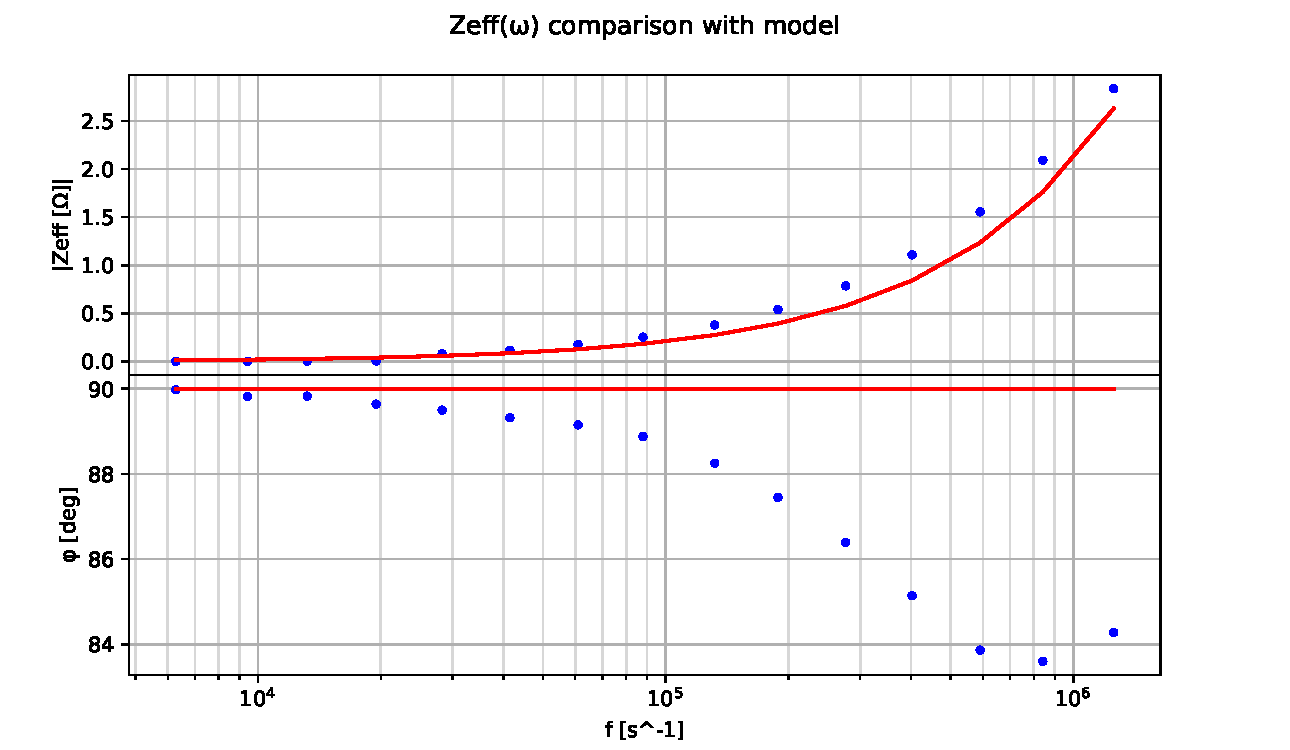
\includegraphics[width=\textwidth]{Figure_15.pdf}
    
    \caption{Confronto tra $Z_{eff}$ in blu e l'impedenza del coefficiente di mutua induzione in rosso.}
    \label{fig:zeff}
\end{figure}
La deviazione della fase, seppur di pochi gradi, pu\'o essere attribuita ad effetti di ordine maggiore qui non presi in considerazione.\\

Si analizza ora l'andamento dell'induzione all'aumentare della distanza, figura \ref{fig:brut}.
\begin{figure}[H]
	\centering
    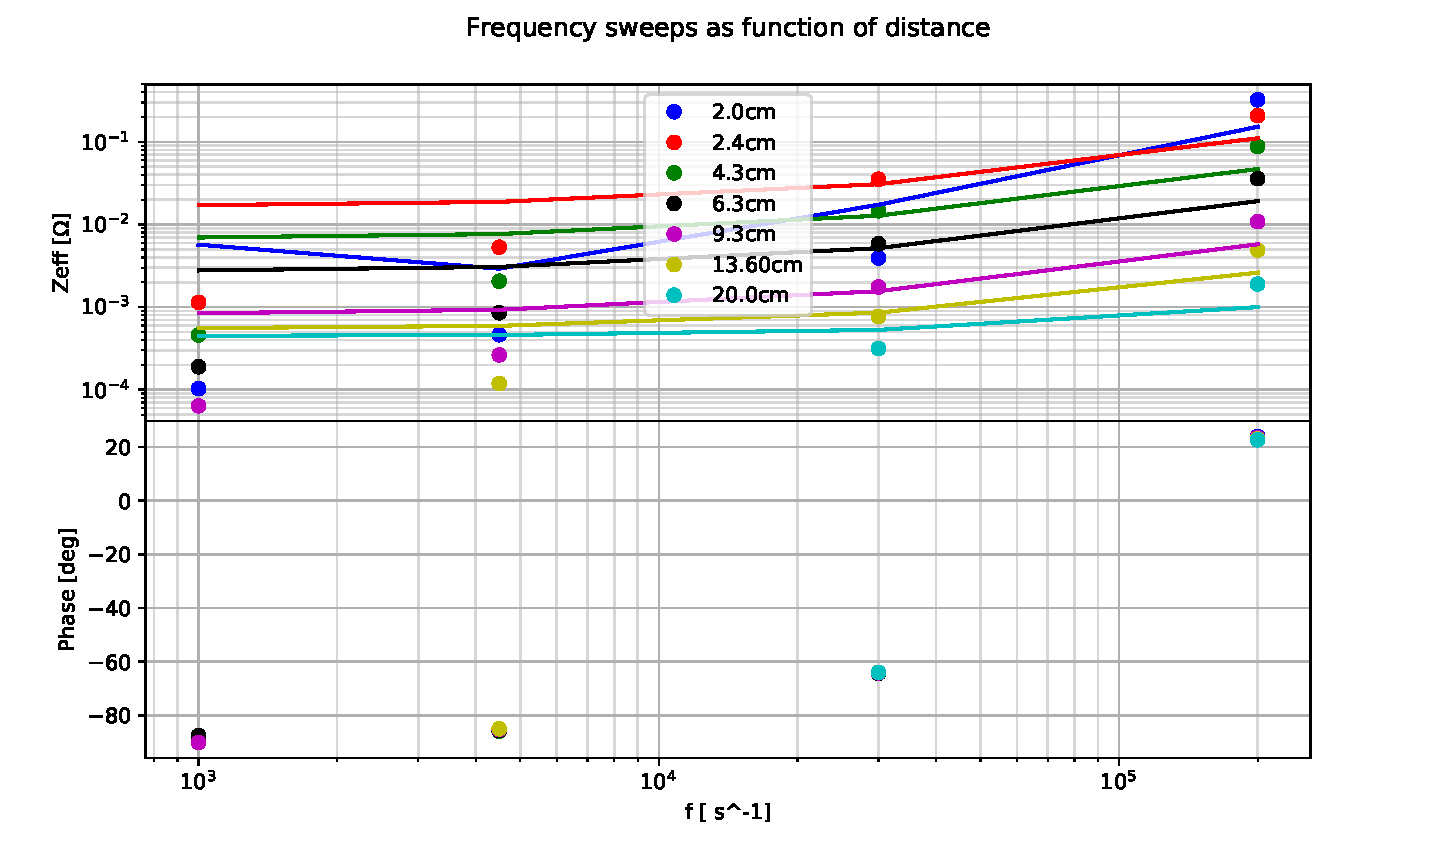
\includegraphics[width=\textwidth]{Figure_16.pdf}
    
    \caption{Confronto a varie distanze in funzione della frequenza.}
    \label{fig:brut}
\end{figure}
L'andamento della fase non \'e quello aspettato e dovrebbe essere indagato pi\'u a fondo con nuovi dati ed un nuovo setup, tuttavia mi aspetto che il modulo aumenti con la frequenza come \'e successo precedentemente.\\
Viene ora scelta la frequenza di $200\ \si{\kilo\hertz}$ per la quale ho dati a tutte le distanze e viene mostrato in figura \ref{fig:r3} il coefficiente di mutua induzione calcolato dalle misure di tensione in entrata ed in uscita comparato all'induzione che un dipolo magnetico esercita su una spira che si muove lungo l'asse di simmetria.\\
\begin{figure}[h]
	\centering
    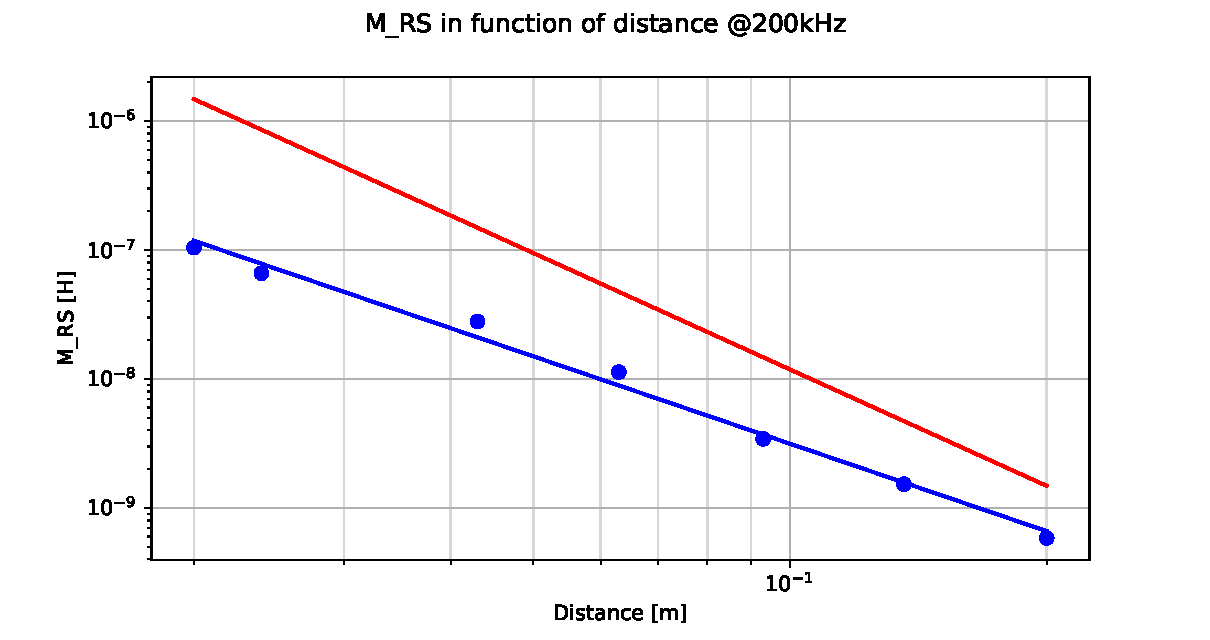
\includegraphics[width=\textwidth]{Figure_17.pdf}
    
    \caption{Mutua induzione in funzione della distanza.}
    \label{fig:r3}
\end{figure}
In rosso \'e mostrato il modello teorico:
\begin{gather}
	r=8.75\ \si{\milli\meter} \\
	\Sigma = \pi r^2 \\
	m_S=N i_S \Sigma \\
	B_{asse}=\frac{\mu_0 2 m_S}{4 \pi d^3} \\
	\Phi_B = N B_{asse} \Sigma \\
	M_{RS} = \frac{\Phi_B}{i_S}
\end{gather}
In blu si mostrano i punti sperimentali assieme alla loro regressione lineare sulla scala logaritmica:
\begin{gather}
	M_{RS,log}=\log (M_{RS}) \qquad d_{log}=\log (d)\\
	M_{RS,log,fit}=A+B d_{log} \\
	M_{RS,fit} = \exp (M_{RS,log,fit}) \\
	A=-24.76 \qquad B=-2.25
\end{gather}
Come si pu\'o vedere non solo i punti sperimentali sono traslati in basso ma il coefficiente $B$ rappresentante l'esponente della distanza \'e diverso da $-3$ come compare nella formula teorica sopra esposta, questo provoca un ulteriore incongruenza. Questo tipo di incongruenze sono dovute al fatto che stiamo usando per il modello l'"approssimazione di dipolo magnetico" la quale \'e valida solamente su grandi distanze mentre a piccole distanze non segue pi\'u una legge di tipo $\propto 1/d^3$. Inoltre la spira ha un certo spessore e parte del flusso entrante al primo giro di essa esce prima di concatenarsi a quelle successive provocando quindi una diminuzione del coefficiente di mutua induzione come mostrato nel grafico. Notare inoltre che all'aumentare della distanza la legge teorica raggiunge la regressione effettuata sui punti sperimentali come ci si aspetta.\\